%|--------------------------------------|
%| Introduction to the EAGLE simulation |
%|--------------------------------------|
\section{The EAGLE simulation suite}
\label{eagle_sim_suite}

%|----------------------|
%| Table of simulations |
%|----------------------|
\begin{table*}
\small
\begin{center}
\renewcommand{\arraystretch}{1.5}
\begin{tabular}{lrrrrrrrrrr}
\hline
Identifier & L & N & $m_{\text{g}}$ & $m_{\text{dm}}$ & $\epsilon_{\text{com}}$ & $\epsilon_{\text{phys}}$ & $n_{\text{H,0}}$ & $n_{\text{n}}$ & $C_{\text{visc}}$ & $\Delta \text{T}_{\text{AGN}}$\\
& [cMpc] &  & [M$_{\odot}$] & [M$_{\odot}$] & [ckpc] & [pkpc] & [cm$^{-3}$] & & & [K]\\
\hline\hline
Ref-L0025N0376 & 25 & $2{\times}376^{3}$ & $1.81{\times}10^{6}$ & $9.70{\times}10^{6}$ & 2.66 & 0.70 & 0.67 & 2/ln10 & 2$\pi$ & $10^{8.5}$\\
Ref-L0025N0752 & 25 & $2{\times}752^{3}$ & $2.26{\times}10^{5}$ & $1.21{\times}10^{6}$ & 1.33 & 0.35 & 0.67 & 2/ln10 & 2$\pi$ & $10^{8.5}$\\
Recal-L0025N0752 & 25 & $2{\times}752^{3}$ & $2.26{\times}10^{5}$ & $1.21{\times}10^{6}$ & 1.33 & 0.35 & 0.25 & 1/ln10& 2$\pi{\times} 10^3$ & $10^{9.0}$\\
Ref-L0050N0752 & 50 & $2{\times}752^{3}$ & $1.81{\times}10^{6}$ & $9.70{\times}10^{6}$ & 2.66 & 0.70 & 0.67 & 2/ln10& 2$\pi$ & $10^{8.5}$\\
AGNdT9-L0050N0752 & 50 & $2{\times}752^{3}$ & $1.81{\times}10^{6}$ & $9.70{\times}10^{6}$ & 2.66 & 0.70 &0.67& 2/ln10& 2$\pi{\times} 10^2$ & $10^{9.0}$\\
Ref-L0100N1504 & 100 & $2{\times}1504^{3}$ & $1.81{\times}10^{6}$ & $9.70{\times}10^{6}$ & 2.66 & 0.70 & 0.67 & 2/ln10& 2$\pi$ & $10^{8.5}$\\
\hline
\end{tabular}
\end{center}
\caption{Parameters describing the available simulations. From
  left-to-right the columns show: simulation name suffix; comoving box size;
  total number of particles; initial baryonic particle mass; dark matter
  particle mass; comoving Plummer-equivalent gravitational softening length;
  maximum physical softening length and the subgrid model parameters that vary:
  $n_{\text{H,0}}$, $n_{\text{n}}$, $C_{\text{visc}}$ and $\Delta
  \text{T}_{\text{AGN}}$ (see section 4 of \citet{Schaye2015} for an explanation of their
  meaning).}
\label{table_simulation_list}
\end{table*}

The \eagle simulation suite is a set of cosmological hydrodynamical simulations
in cubic, periodic volumes ranging from 25 to 100 comoving megaparsecs (cMpc) per side that
track the evolution of both baryonic (gas, stars and massive black holes) and
non-baryonic (dark matter) elements from a starting redshift of $z = 127$ to the
present day. All simulations adopt a flat $\Lambda$CDM cosmology with parameters
taken from the \emph{Planck} mission \citep{Planck2013} results: $\Omega_\Lambda
= 0.693$, $\Omega_m = 0.307$, $\Omega_b = 0.04825$, $\sigma_8 = 0.8288$, $n_s =
0.9611$, $Y=0.248$ and $H_0 = 67.77$ km s$^{-1}$ Mpc$^{-1}$ (i.e. $h=0.6777$). The initial
conditions were generated using second-order Lagrangian perturbation theory
\citep{Jenkins2010} and the phase information is taken from the public {\sc
  panphaisa} Gaussian white noise field \citep{Jenkins2013}. Full details of how
the ICs were made are given in Appendix B of \cite{Schaye2015}. The simulation
suite was run with a modified version of the \gadget-3 Smoothed Particle
Hydrodynamics (SPH) code \citep[last described by][]{Springel2005},
and includes a full treatment of gravity and hydrodynamics. The modifications to
the SPH method are collectively referred to as \anarchy (Dalla Vecchia,
(\textit{in prep.}), see also Appendix A of \cite{Schaye2015} and
\cite{Schaller2015b}), and use the ${\cal C}_2$ kernel of \cite{Wendland1995},
the pressure-entropy formulation of SPH of \citet{Hopkins2013}, the time-step
limiters introduced by \cite{Durier2012}, the artificial viscosity switch of
\cite{Cullen2010} and a weak thermal conduction term of the form proposed by
\cite{Price2008}.  The effects of this state-of-the-art formulation of SPH on
the galaxy properties is explored in detail by \cite{Schaller2015b}.

\subsection{Subgrid model}
Processes not resolved by the numerical scheme are implemented as subgrid source
and sink terms in the differential equations. For each process, schemes were
adopted that are as simple as possible and that only depend on the local
hydrodynamic properties. This last requirement differentiates \eagle from most
other cosmological, hydrodynamical simulation projects
\citep[e.g.][]{Oppenheimer2010,Puchwein2013,Vogelsberger2014,Khandai2015} and
ensures that galactic winds develop without pre-determined mass loading factors
and directions, without any direct dependence on halo or dark matter
properties. 

The simulation tracks the time-dependent stellar mass loss due to winds from
massive stars and AGB stars, core collapse supernovae and type Ia supernovae
\citep{Wiersma2009b}. Radiative cooling and heating is implemented
element-by-element following \cite{Wiersma2009a}. Cold dense gas is prevented
from artificial fragmentation by implementing an effective temperature pressure
floor as described by \cite{Schaye_DallaVecchia2008}. Star formation is
implemented stochastically following the pressure-dependent Kennicutt-Schmidt
relation \citep{Schaye_DallaVecchia2008}, with the inclusion of a
metal-dependent star formation threshold designed to track the transition from a
warm, atomic to an unresolved, cold, molecular gas phase, as proposed by
\cite{Schaye2004}. The initial stellar mass function is that given by
\cite{Chabrier2003}. Feedback from star formation is implemented thermally and
stochastically following the method of \cite{DallaVecchia_Schaye2012}. Seed
black holes are placed in haloes greater than a threshold mass of $10^{10}\Msol
/ h$ and tracked following the methodology of \cite{Springel2005a} and
\cite{Booth_Schaye2009}. Gas accretion onto black holes follows a modified
version of the Bondi-Hoyle accretion rate, described by \citep[][, but modified
  as described by \cite{Schaye2015}]{Guevara2013}, and feedback is implemented
following the stochastic AGN heating scheme described by \cite{Schaye2015} and
making use of the energy threshold of \cite{Booth_Schaye2009}. The details of
the implementation and parametrisation of these schemes are motivated and
described in detail by \cite{Schaye2015}.

Because of our limited understanding of these processes and because of the
limited resolution of the simulations, the subgrid source and sink terms involve
free parameters whose values must be determined by comparison of the simulation
results to a subset of the observational data. In the case of \eagle, the
subgrid parameters were calibrated for feedback from star formation and AGN by
using three properties of galaxies at redshift $z=0$, specifically the galaxy
stellar mass function, the galaxy size -- stellar mass relation, and the black
hole mass -- stellar mass relation. The calibration strategy is described in
detail by \citet{Crain2015} who also presented additional simulations to
demonstrate the effect of parameter variations.

Once the simulations have been calibrated using a subset of the observational
data, they can be validated by comparison to additional datasets.  Studies have
so far shown that the simulations broadly reproduce a variety of other
observables such as the $z=0$ Tully-Fisher relation, specific star formation
rates and the column density distribution of intergalactic \CIV and \OVI
\citep{Schaye2015}, the \HI and $\rm{H}_2$ properties of galaxies \citep[Bah\'e
  et al. {\textit submitted},][]{Lagos2015}, the column density distribution of
intergalactic metals \citep{Schaye2015}, galaxy rotation curves
\citep{Schaller2015a}, the $z=0$ luminosity function and colour-magnitude
diagram \citep{Trayford2015}, the evolution of the galaxy stellar mass function
\citep{Furlong2015} and the high-redshift \HI column density distribution
\citep{Rahmati2015}.

\subsection{The simulations in the database}
Table~\ref{table_simulation_list} summarises the simulations that have been
incorporated into the database, including the comoving cubic box length,
baryonic and non-baryonic particle masses and gravitational softening
lengths. Together these parameters determine the dynamic range and resolution
that can be achieved by the simulation. The simulation name includes a suffix to
indicate the simulation box length in comoving megaparsecs (e.g. L0100) and the
cube root of the initial number of particles per species
(e.g. N1504). Simulations with the same subgrid model as the primary run
(L0100N1504) are denoted with the prefix \dquotes{Ref-}. As discussed in
\citet{Schaye2015}, the \dquotes{Recal-} higher-resolution simulation uses
values of the subgrid parameters that have been recalibrated following the same
procedure used for the reference simulation to improve the fit to the $z=0$
galaxy stellar mass function, allowing the user to test the \emph{weak}
convergence of the code\footnote{As discussed in Section~\ref{caveats},
  performing convergence tests is strongly encouraged.}. See \cite{Schaye2015}
for definitions and discussion of the concepts of weak and strong
convergence. Note that Recal-L0025N0752 should be compared to the Ref-L0025N0376
calculation to ensure that the same range of halo mass is sampled in both cases,
eliminating differences due to the simulation volume. To a similar end, the
Ref-L0025N0752 model is provided to allow the user to test the \emph{strong}
convergence of the results. This simulation uses all the subgrid parameters of
the reference model but at a higher mass resolution. All the 25~cMpc volumes
share the same large-scale initial fluctuations, so that objects appear in
(approximately) the same spatial locations in all three runs.

Finally, the database also includes the additional simulation AGNdT9-L0050N0752
that uses a higher AGN heating temperature and increased black hole accretion
viscosity parameter, $C_{\text{visc}}$. As discussed by \cite{Schaye2015}, this
results in a better match to the properties of diffuse gas in galaxy group
haloes, but has only a small effect on the properties of galaxies. This
simulation uses the same initial phases as the Ref-L0050N0752 model, allowing
objects to be matched.

\subsection{Halo, subhalo and galaxy identification}

The raw particle data themselves are not required for many comparisons with
observations. In order to reduce the volume of data to be downloaded and
simplify analysis, we process the simulation outputs individually to locate bound
structures which we identify with galaxies and their associated dark matter
haloes. The processing steps are described in detail by \cite{Schaye2015}. In
brief, overdensities of dark matter are identified using the
\dquotes{Friends-of-Friends} (FoF) method \citep{Davis1985} adopting a linking
length of 0.2 times the average inter-particle spacing. Baryonic particles are
then assigned to the same FoF-halo as their closest dark matter
neighbour. Self-bound \dquotes{subhaloes}, which can contain both baryonic and
dark matter, are later identified using the \subfind algorithm
\citep{Springel2001,Dolag2009} using all particle species.

It is important to note that particles are not shared between subhaloes so that
the correspondence between particles and subhaloes is unique. We identify the
baryonic component of each subhalo with a galaxy and will refer to them as such
from now on. Resolved subhaloes, always have a clear central concentration and
there is a clear identification between the galaxies in the simulations and
galaxies that would be identified in observational studies. Note that small
subhaloes, especially at high redshift, may not contain any stars or even gas
but will still be present in the catalogues. A FoF halo may contain several
subhaloes (or sub-groups in the \subfind terminology); we define the subhalo
that contains the particle with the lowest value of the gravitational potential
to be the \emph{central galaxy} while any remaining subhaloes are classified as
\emph{satellite galaxies} (denoted \texttt{SubGroupNumber} $= 0$ and
\texttt{SubGroupNumber} $> 0$ respectively in the database nomenclature, see
below).

The stellar mass assigned to a galaxy may include diffuse particles at a large
distance. Such particles make up the intra-cluster/intra-group light and would
not normally be included in a galaxy's photometry. We therefore also include
aperture-based measurements in the database. 

Exceptionally, \subfind may identify an internal high-density component of a
galaxy as a distinct subhalo. Such spurious identifications are discussed in
Sec.~\ref{caveats} and are labelled in the main database table with the field
{\tt Spurious}.

For each simulation we release 29 snapshot outputs between redshift $20$ and $0$
(the full list of released output redshifts is given in the Appendix table
\ref{table:snapshot_list}). We later analyse the properties of each subhalo in
post-processing in order to calculate galaxy and subhalo properties, such as
stellar masses, galaxy sizes, star formation rates and luminosities. Each
subhalo and hence each galaxy is assigned an index, its \HaloID, that allows one
to identify an object uniquely both in space and time. Note that since the
\HaloID is unique to a particular output redshift, a galaxy will change its
\HaloID over time. The 29 catalogues of galaxies are then linked through time
via a galaxy merger tree, allowing one to track the evolution of a galaxy
(through the evolution of its \HaloID) with time.  The construction and
structure of these trees is presented in Section \ref{subsection:merger_trees}.

\subsection{Integrated quantities}
At each redshift the galaxies are processed one-by-one to produce integrated
quantities from the raw particle information. These are the quantities stored in
the different tables of the database.

For the simplest quantities, such as galaxy mass, metallicity or star formation
rate, the post-processing only involves a simple summation over the particles
but other quantities, such as luminosities in various filters, require much more
involved calculations. The full list of quantities present in the database,
together with a description of the post-processing operations performed, is
given in \ref{appendix_quantities}. To allow for an easier comparison with
observational measurements, masses, star formation rates and velocity
dispersions are also computed within fixed spherical apertures.

\subsection{Mock gri images}

\begin{figure*}
\centering
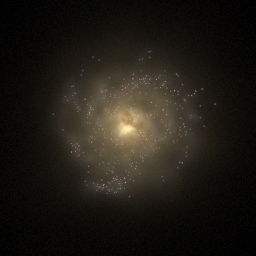
\includegraphics[width=0.32\textwidth]{figures/galface_16116800.png}
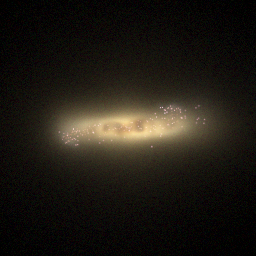
\includegraphics[width=0.32\textwidth]{figures/galedge_16116800.png}
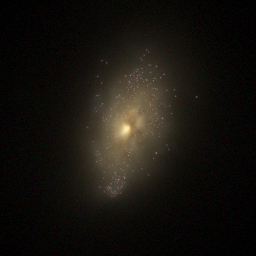
\includegraphics[width=0.32\textwidth]{figures/galrand_16116800.png}
\caption{Mock $gri$ images of a galaxy at $z=0.1$ as available in the database. The left,
  central and right panels correspond to the {\tt Image\_face}, {\tt
    Image\_edge} and {\tt Image\_box} views (in the database nomenclature) of
  the same simulated galaxy ({\tt GalaxyID}$~=16116800$ in the Ref-L0100N1504
  simulation). The images are 60~pkpc on a side. Note the clear presence of a
  bulge, of dust absorption and of spiral arms.}
\label{fig:mockImage}
\end{figure*}

For visualisation purposes, images are provided for galaxies with 30 physical
kpc (pkpc) aperture stellar masses $> 10^{10} {\rm M}_\odot$. Images are
generated from mock observations made using the {\sc skirt} code \citep{Baes03,
  Camps15}, with \textsc{galaxev} \citep{BC03} and \textsc{mappings iii}
\citep{Groves08} spectra to represent star particles and young H\textsc{ii}
regions respectively, as described by Trayford et.al., (\textit{in prep.}). A
square field of view of 60~pkpc on a side is used for observations in the SDSS
$gri$ bands \citep{SDSSfilters}, with the galaxy spectra red-shifted to $z =
0.1$ to approximate SDSS colours. No artificial seeing is added to the
images. Each galaxy above the stellar mass threshold is observed \textit{face-}
and \textit{edge-on} to the galactic plane, defined using the stellar angular
momentum vector within 30~pkpc. A `\textit{box}' projection is also provided,
with galaxies viewed down the simulation z-axis and the horizontal and vertical
image axes corresponding to the simulation $x$ and $y$ axes respectively. The
three-colour $gri$ images are prepared from the virtual {\sc skirt} observations
adopting the method of \citet{Lupton04}. Figure \ref{fig:mockImage} shows these
three images for the same example galaxy.
